% Appendix: Reward Signal Robustness Across Judges
% Validates that the paper's conclusions are robust to evaluator choice.

\section{Reward Signal Robustness (Three-Judge Validation)}
\label{sec:judge_robustness}

All main-paper experiments use DeepSeek-R1 as the sole evaluator.
A natural concern is whether the paper's conclusions---the relative
ordering of methods and the qualitative behaviour of the router---are
artefacts of this particular judge.  We address this with a
three-judge validation aimed at a single question: would the paper's
conclusions change with a different evaluator?

\subsection{Setup}

We draw a stratified random sample of $n = 2{,}000$ prompts from the
12{,}000-prompt benchmark, preserving proportional representation of
all source benchmarks.  Each prompt has existing responses from all
three candidate models (Llama-3.1-8B, Mistral-Large-2512,
Gemini-2.5-Pro), yielding $6{,}000$ (prompt, model) evaluation pairs.
We re-evaluate these fixed responses---no new model outputs---with two
supplementary judges chosen for provider diversity: GPT-4.1-mini
(OpenAI) and Claude-3.7-Sonnet (Anthropic).

All three judges receive the same structured chain-of-thought
evaluation prompt (Figure~\ref{fig:judge_prompt}); DeepSeek-R1
additionally receives a brevity instruction to limit its CoT
verbosity.  The composite reward is a weighted average
$r = 0.4\,s_{\text{reason}} + 0.3\,s_{\text{instr}} +
0.3\,s_{\text{comm}}$.  The judge panel spans three independent
providers (DeepSeek, OpenAI, Anthropic), none of which overlaps with
the routed model providers (Meta, Mistral, Google).

\begin{figure*}[t]
\centering
\begingroup
\fontsize{5.6}{6.2}\selectfont
\begin{verbatim}
SYSTEM:
You are a Discriminative Router Judge. Your goal is to evaluate
how well an LLM response addresses the given prompt.

Score on three continuous dimensions (0.0-1.0). Use the FULL
range; do NOT default to 0 or 1.

1. Reasoning Quality (40%) - How sound is the reasoning?
   0.9-1.0  Flawless; every step correct and clearly justified.
   0.7-0.8  Sound overall; minor inefficiency or a trivial
            error that does not change the conclusion.
   0.5-0.6  Partially correct; approach is reasonable but
            important steps are wrong or missing.
   0.3-0.4  Weak; only fragments of correct logic.
   0.0-0.2  No coherent reasoning, or completely wrong approach.
   If the prompt needs no multi-step reasoning, score factual
   accuracy and depth of explanation.

2. Instruction Following (30%) - Were all explicit and implicit
   constraints satisfied?
   0.9-1.0  Every constraint followed precisely.
   0.7-0.8  All major constraints met; one minor instruction
            partially missed.
   0.5-0.6  Some important instructions missed or only
            partially addressed.
   0.3-0.4  Multiple instructions ignored or misinterpreted.
   0.0-0.2  Response largely ignores the prompt's requirements.

3. Communication Quality (30%) - How clear, well-structured,
   and useful is the response?
   0.9-1.0  Exceptionally clear, well-organized, appropriate
            detail.
   0.7-0.8  Clear and competent; minor improvements possible.
   0.5-0.6  Adequate but noticeably unclear, verbose, or poorly
            organized.
   0.3-0.4  Hard to follow; significant clarity issues.
   0.0-0.2  Unintelligible, unhelpful, or inappropriate tone.

Format your response EXACTLY as follows:

## Reasoning
<Concise chain-of-thought analysis>

## Reasoning Quality
<0.0 to 1.0>

## Instruction Following
<0.0 to 1.0>

## Communication Quality
<0.0 to 1.0>

USER:
PROMPT: {prompt}

RESPONSE: {response}
\end{verbatim}
\endgroup
\caption{Structured CoT evaluation prompt sent to all three judges.
The composite reward is
$r = 0.4\,s_{\text{reason}} + 0.3\,s_{\text{instr}} + 0.3\,s_{\text{comm}}$.
For DeepSeek-R1 only, the system message appends: ``\texttt{IMPORTANT:
Keep the \#\# Reasoning section to 3--5 sentences.  Be direct---identify
errors or confirm correctness, then move to scoring.}''
Temperature is set to 0 for all judges.}
\label{fig:judge_prompt}
\end{figure*}

\subsection{Population-Level Agreement}

The bandit's converged policy depends on the expected reward ordering
$\mathbb{E}[r(x, a)]$ across arms, not on individual prompt scores.
If this ordering is preserved across judges, the converged policy is
invariant to evaluator choice.

\begin{table}[h]
\centering
\caption{Expected reward ordering under each judge.  All three judges
produce the identical ranking Gemini-Pro $>$ Mistral-Large $>$ Llama-8B,
with every pairwise difference significant (Bonferroni-corrected
bootstrap CI excludes zero; 9 comparisons, $B = 10{,}000$,
$n = 2{,}000$).}
\label{tab:expected_ordering}
\small
\resizebox{\columnwidth}{!}{%
\begin{tabular}{lccc}
\toprule
\textbf{Judge} & \textbf{Gemini-Pro} & \textbf{Mistral-Large} & \textbf{Llama-8B} \\
\midrule
DeepSeek-R1       & \jrROneGeminiMean{} & \jrROneMistralMean{} & \jrROneLlamaMean{} \\
GPT-4.1-mini      & \jrGPTGeminiMean{} & \jrGPTMistralMean{} & \jrGPTLlamaMean{} \\
Claude-3.7-Sonnet & \jrClaudeGeminiMean{} & \jrClaudeMistralMean{} & \jrClaudeLlamaMean{} \\
\bottomrule
\end{tabular}
}
\end{table}

Table~\ref{tab:expected_ordering} shows that all three judges rank
the models identically: Gemini-Pro $>$ Mistral-Large $>$ Llama-8B.
Every pairwise expected-reward gap has the same sign, with all nine
Bonferroni-corrected bootstrap CIs excluding zero (narrowest lower
bound 0.0046; 9 comparisons, $B = 10{,}000$).
Gap-conditioned Kendall's~$W$ (Table~\ref{tab:routing_diagnostics})
reaches 0.71 on prompts with large inter-model gaps, indicating that
the conditional ordering $\mathbb{E}[r(x,a) \mid x]$ is also largely
preserved where routing decisions matter most.

Because all main-paper comparisons are within-judge (same R1 rewards,
same R1 oracle), judge choice can change the magnitude of regret
differences but not their sign.  R1's oracle lift (0.031 per step) is
the largest among the three judges (0.016--0.020 for the supplementary
judges), so main-paper effect sizes correspond to the most favourable
case for adaptive routing; all qualitative conclusions hold under every
judge tested.

\paragraph{Cross-judge routing regret.}
Even where per-prompt routing decisions differ, the practical cost is
small.  Following R1's oracle policy and evaluating with the other
judges' scores yields ${\geq}97.4\%$ of their own oracle reward
(Table~\ref{tab:cross_regret}).  The reverse is worse: following
GPT-4.1-mini's or Claude's oracle and evaluating with R1 captures only
$95.8\%$ of R1's oracle reward.  The asymmetry is partly mechanical:
judges with smaller inter-model gaps inflate capture fractions for any
routing policy, while R1's larger gaps penalise misrouting more
heavily.

\begin{table}[h]
\centering
\caption{Cross-judge routing evaluation.  Each cell reports the mean
reward achieved by following the row judge's oracle, evaluated by the
column judge's scores.  Parenthetical values show the fraction of the
column judge's own oracle reward captured ($B = 10{,}000$ bootstrap
resamples).}
\label{tab:cross_regret}
\small
\resizebox{\columnwidth}{!}{%
\begin{tabular}{lccc}
\toprule
\textbf{Train $\downarrow$ / Eval $\rightarrow$}
    & \textbf{R1} & \textbf{GPT-4.1-mini} & \textbf{Claude-3.7} \\
\midrule
R1
    & \jrCrossROneROneMean{} (100\%) & \jrCrossROneGPTMean{} (\textbf{\jrCrossROneGPTCapture\%}) & \jrCrossROneClaudeMean{} (\textbf{\jrCrossROneClaudeCapture\%}) \\
GPT-4.1-mini
    & \jrCrossGPTROneMean{} (\jrCrossGPTROneCapture\%) & \jrCrossGPTGPTMean{} (100\%) & \jrCrossGPTClaudeMean{} (\jrCrossGPTClaudeCapture\%) \\
Claude-3.7-Sonnet
    & \jrCrossClaudeROneMean{} (\jrCrossClaudeROneCapture\%) & \jrCrossClaudeGPTMean{} (\jrCrossClaudeGPTCapture\%) & \jrCrossClaudeClaudeMean{} (100\%) \\
\bottomrule
\end{tabular}
}
\end{table}
\vspace{6pt}

Panel averaging~\cite{zheng2023judging} compresses routing margins:
averaging the three judges shrinks the mean inter-model gap from
$0.0485$ (R1 alone) to $0.0338$ (30\% compression), halving the
fraction of actionable prompts (31\% vs.\ 17\% at a 0.05 threshold).
Z-score calibration~\cite{hedges1985statistical} and multi-judge
aggregation methods such as PoLL~\cite{verga2024poll} and
CARE~\cite{zhao2025care} recover $< 3$ percentage points of this
compression, indicating genuine inter-judge disagreement rather than
pure scale mismatch.  R1 alone provides the largest margins and the
lowest per-evaluation cost.

\subsection{Per-Prompt Agreement}

Table~\ref{tab:judge_agreement} reports per-response agreement using
distribution-independent metrics robust to ceiling-compressed rewards
(most scores in $[0.8, 1.0]$).  Spearman's $\rho$ (0.633--0.658) and
Kendall's $\tau_b$ (0.528--0.547) indicate moderate rank agreement;
mean absolute deviation is ${\approx}0.075$ and Bland--Altman limits
of agreement remain within roughly $\pm 0.3$.  This level of
LLM-as-judge noise is expected, and the key point is that it preserves
population-level ordering and routing policies.

\begin{table}[h]
\centering
\caption{Per-response agreement with DeepSeek-R1 ($6{,}000$ scored pairs
per judge).  All measures are rank-based or distribution-independent to avoid
attenuation from ceiling-compressed rewards.}
\label{tab:judge_agreement}
\small
\resizebox{\columnwidth}{!}{%
\begin{tabular}{lcc}
\toprule
\textbf{Metric} & \textbf{GPT-4.1-mini} & \textbf{Claude-3.7-Sonnet} \\
\midrule
Spearman's $\rho$            & \textbf{\jrGPTSpearman} & \jrClaudeSpearman{} \\
Kendall's $\tau_b$           & \textbf{\jrGPTKendall} & \jrClaudeKendall{} \\
MAD                          & \textbf{\jrGPTMAD} & \jrClaudeMAD{} \\
Mean bias (judge $-$ R1)     & $+\jrGPTBias$ & $\jrClaudeBias$ \\
95\% Bland--Altman LoA       & [$\jrGPTBALo$, $+\jrGPTBAHi$] & [$\jrClaudeBALo$, $+\jrClaudeBAHi$] \\
\bottomrule
\end{tabular}
}
\end{table}

\paragraph{Gap-conditioned concordance.}
Per-prompt best-model agreement with R1 is ${\sim}50\%$ overall, but
disagreements cluster on prompts where all models are nearly tied.
Table~\ref{tab:routing_diagnostics} shows that when R1's inter-model
gap is $< 0.05$ (30\% of prompts), Kendall's $W = 0.17$ and
best-model agreement is 48--58\%; when the gap is $\geq 0.20$ (37\%
of prompts), $W$ rises to 0.57--0.71 and best-model agreement to
50--58\%.  In the low-gap region, choosing the ``wrong'' model costs
at most 0.05 reward---less than per-response judge noise
(MAD ${\approx} 0.075$)---so disagreement is concentrated where it is
cheap.

\begin{table}[h]
\centering
\caption{Routing agreement conditioned on R1's inter-model gap.
Kendall's~$W$ measures three-judge concordance on the full model ranking.
Agreement is strong where the routing decision has the greatest reward
impact (gap $> 0.20$) and weak where all models produce near-identical
quality (gap $< 0.05$).  Conditioning on R1's gap bins when validating
R1 can introduce selection bias; we verify in the reproducibility code
that the same monotonic trend holds when conditioning on the consensus
(panel-median) gap.}
\label{tab:routing_diagnostics}
\small
\resizebox{\columnwidth}{!}{%
\begin{tabular}{lrccc}
\toprule
& & & \multicolumn{2}{c}{\textbf{Best-model agr.\ vs.\ R1}} \\
\cmidrule(lr){4-5}
\textbf{R1 gap range} & $n$ & \textbf{Kendall $W$}
    & \textbf{GPT-mini} & \textbf{Claude} \\
\midrule
$[0.00, 0.05)$ & 603  & 0.17 & 57.5\% & 48.3\% \\
$[0.05, 0.10)$ & 367  & 0.29 & 37.6\% & 37.9\% \\
$[0.10, 0.20)$ & 294  & 0.43 & 44.9\% & 39.5\% \\
$[0.20, 0.30)$ & 184  & 0.57 & 53.3\% & 49.5\% \\
$[0.30, 1.00)$ & 552  & 0.71 & 56.3\% & 58.0\% \\
\midrule
\emph{Overall} & 2{,}000 & 0.42 & 51.3\% & 47.9\% \\
\bottomrule
\end{tabular}
}
\end{table}

\subsection{End-to-End Regret Under Alternative Judges}
\label{sec:cross_judge_regret}

We now test whether the bandit's learning dynamics---convergence shape,
sample complexity, and relative method ordering---are preserved when
the reward signal comes from a different judge, by re-running the
bandit simulation under GPT-4.1-mini and Claude-3.7-Sonnet.

\paragraph{Protocol.}
We split the 2{,}000 judge-robustness prompts into a stratified
$\frac{1}{3}$~validation / $\frac{2}{3}$~test partition
(672 / 1{,}328 prompts).  The bandit learns online during the
validation burn-in (no metrics), then cumulative regret is evaluated
on the held-out test split.  To avoid any data-leakage concern, we use
cold start (Tabula Rasa) only---no warmup priors---so this is the
harder test; if the bandit converges from cold start, warm-start
robustness follows.  We compare Tabula Rasa against a Random baseline
(uniform $1/K$) under four budget regimes (unconstrained, tight,
moderate, loose), with 20 seeds per condition.
All three judges share the same hyperparameters
($\alpha = 0.05$, $\gamma = 0.997$), tuned originally on R1;
judge-specific tuning would only improve the supplementary judges'
results, so this choice is conservative.

\paragraph{Results.}
The bandit converges under all three judges.  Under unconstrained
routing (Figure~\ref{fig:cross_judge_regret}), Tabula Rasa achieves
final cumulative regret of $51.0$\,[47.7, 54.4] vs.\
$106.2$\,[104.6, 107.8] for Random under R1 (52\% reduction);
$32.8$ vs.\ $71.9$ under GPT-4.1-mini (54\% reduction); and
$37.6$ vs.\ $97.6$ under Claude (61\% reduction).  All curves are
sublinear with decreasing slope, consistent with progressive learning
of the reward structure regardless of evaluator.

Absolute regret scales with inter-model margins: GPT-4.1-mini's
Random baseline ($71.9$) is 32\% lower than R1's ($106.2$), with
Claude intermediate at $97.6$.  Supplementary/R1 regret ratios are
stable across budget regimes
(GPT: $0.64$\,[0.60, 0.68] to $0.89$\,[0.82, 0.97];
Claude: $0.74$\,[0.70, 0.79] to $0.92$\,[0.87, 1.00]),
confirming proportional compression rather than a structural change in
learning dynamics.  Tabula Rasa confidence intervals are wider than
Random's, reflecting higher run-to-run variance from cold-start
exploration, but the paired difference (Random $-$ Tabula Rasa) is
significant for all three judges.  Under budget constraints, the
qualitative pattern is identical: tighter budgets increase regret, and
loose-budget regret approaches the unconstrained level.

\begin{figure*}[t]
    \centering
    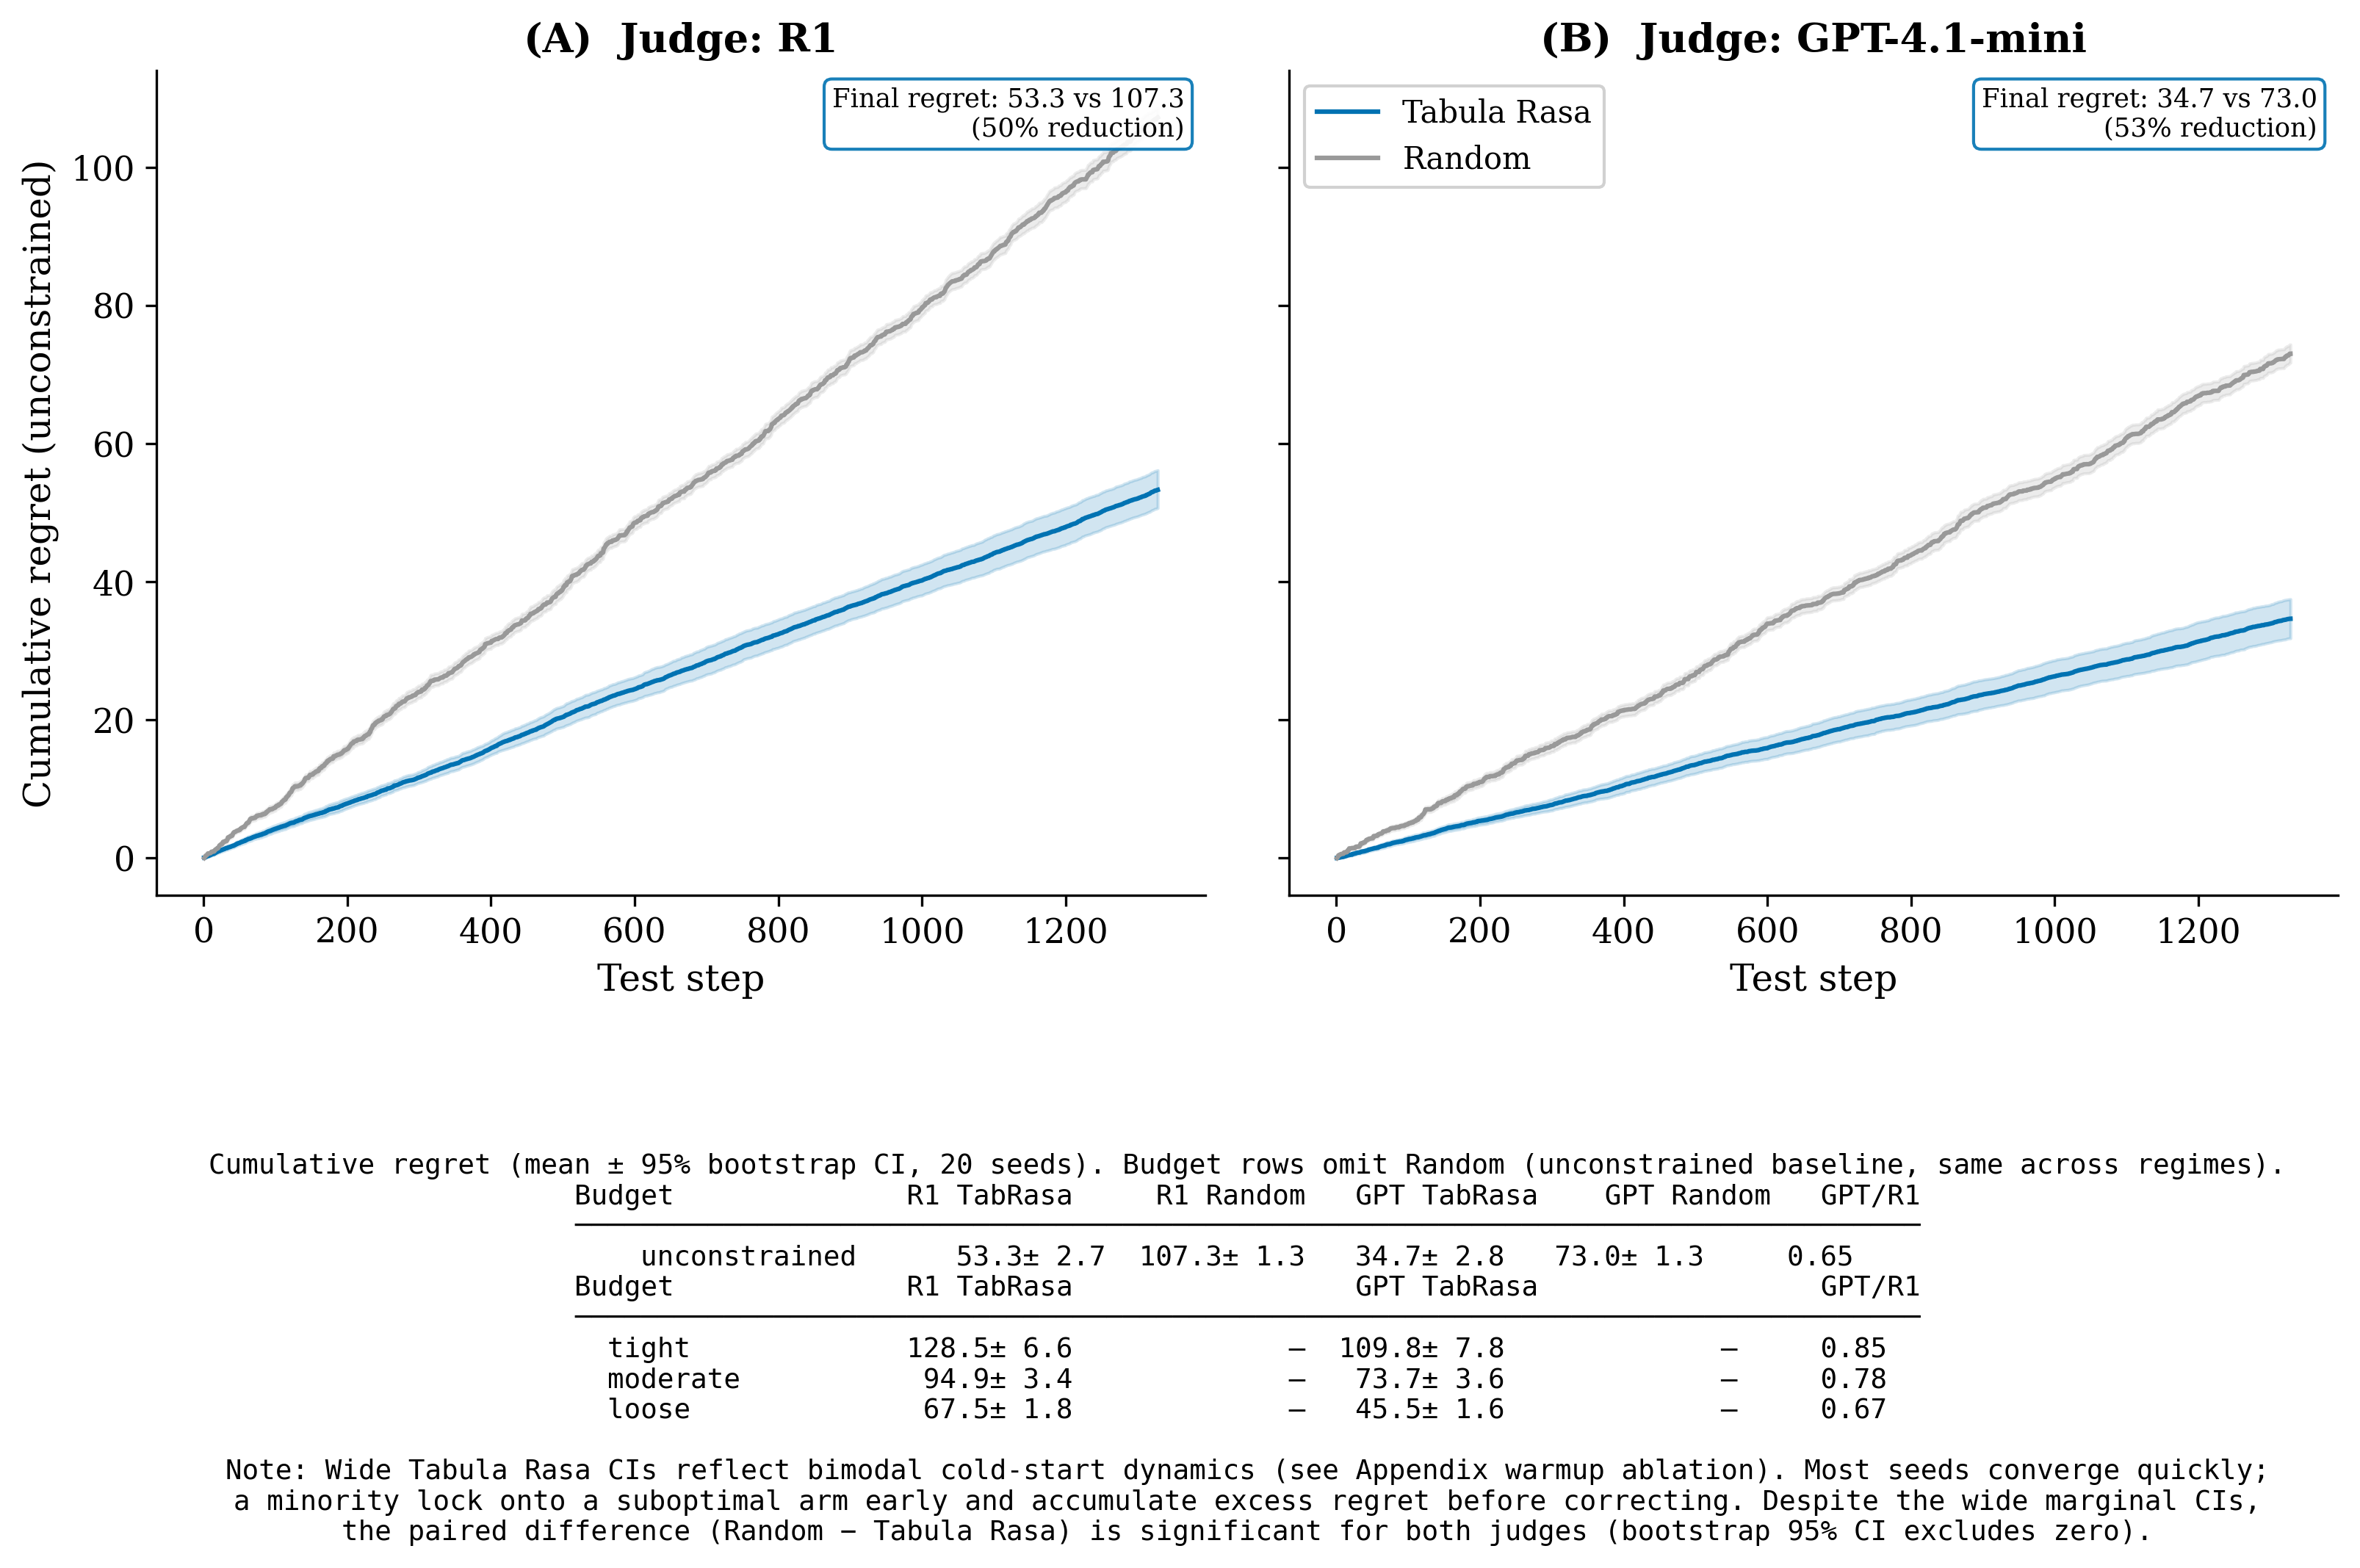
\includegraphics[width=0.92\textwidth]{../experiments/appendix/judge_robustness/results/cross_judge_regret.png}
    \caption{Cold-start bandit regret under three judges (\jrNTest{}
    test prompts drawn from the \jrNSubset{}-prompt judge-robustness sample).
    \textbf{(A)}~R1:
    \jrROneUncReductionPct\% regret reduction.
    \textbf{(B)}~GPT-4.1-mini: \jrGPTUncReductionPct\% reduction.
    \textbf{(C)}~Claude-3.7-Sonnet: \jrClaudeUncReductionPct\% reduction.
    Shaded bands show 95\% bootstrap CIs over \jrNseeds{} seeds.
    Tabula~Rasa bands are wider than the Random baseline's due to higher
    per-seed variance from cold-start exploration.  The paired difference
    (Random~$-$~Tabula~Rasa) is significant for all three judges (bootstrap
    95\% CI excludes zero).  The summary table reports Tabula~Rasa
    cumulative regret (mean $\pm$ 95\% bootstrap CI) across all four budget
    regimes with the supplementary/R1 ratio.}
    \label{fig:cross_judge_regret}
\end{figure*}

\subsection{Summary}

Across three independent judges, the expected reward ordering is
identical (Gemini-Pro $>$ Mistral-Large $>$ Llama-8B;
Table~\ref{tab:expected_ordering}), R1's oracle captures
${\geq}97.4\%$ of other judges' oracle reward
(Table~\ref{tab:cross_regret}), and the bandit's learning dynamics
replicate under both supplementary judges, with regret reductions of
52\%/54\%/61\% (R1/GPT/Claude) under unconstrained routing
(Figure~\ref{fig:cross_judge_regret}).  R1 is therefore well-justified
as the sole evaluator: it provides the largest inter-model margins and
the lowest per-evaluation cost.  Correlating LLM-as-judge scores with
human preferences remains important future work, but it is orthogonal
to the judge-consistency and routing-robustness validated here.
